\chapter{Methodology}
\section{Description of Pipeline}
Based on research into RAG vulnerabilities, there is a clear lack of security measures designed to preserve the privacy of a RAG corpus. This is especially important in fields like healthcare.
As demonstrated in \autocite{zeng2024goodbadexploringprivacy}, private information can be easily extracted by determined attackers through simple prompt injections.
Given that RAG relies on a set of documents as context and its vulnerabilities to RAG, we believe that generating a synthetic document separate from the corpus is sufficient to mitigate most issues.

\section{System Design}
As mentioned, the solution explored in this project consists of an agent-based document synthesis pipeline aimed at preventing raw LLM access to sensitive data.

For all intents and purposes, the pipeline operates in a similar fashion to typical RAG. Upon receiving a query, it fetches document from the RAG corpus then uses the retrieved documents as context in generating a response. However, we include an intermediary step between the information retrieval and inference steps.

Once the documents are retrieved, a  secondary LLM extracts only the necessary information from the documents retrieved. For instance, we may retrieve a medical record consisting of different medical readings for a query about a patient's blood pressure readings. In this example, we aim for the LLM to extract only the blood pressure readings from this document.

With the information retrieved, we use an agent-based approach to modify the information. In order to further distance the information from the original record, we apply the following steps.

Firstly, we remove any PII that may appear in the information. We consider the following as PII: names, ages, contact number and address. The LLM will remove, or replace with pseudonyms, any appearance of PII.

Secondly, we manipulate the data that appears in the information to generalise the record. Numbers are rounded, and converted to ranges if multiple readings of the same type occur.

Finally, to ensure that the LLM treats the synthesized information as relevant context, we modify the original query based on the synthetic information. It should be able to generate the same output as a model operating solely on RAG.

Once it has gone through this step, we pass the synthesized query and information to the primary LLM to generate a response.

Refer to figure \ref{fig:SynthLLMRAG} for a visualization of the system design.

\begin{figure}
	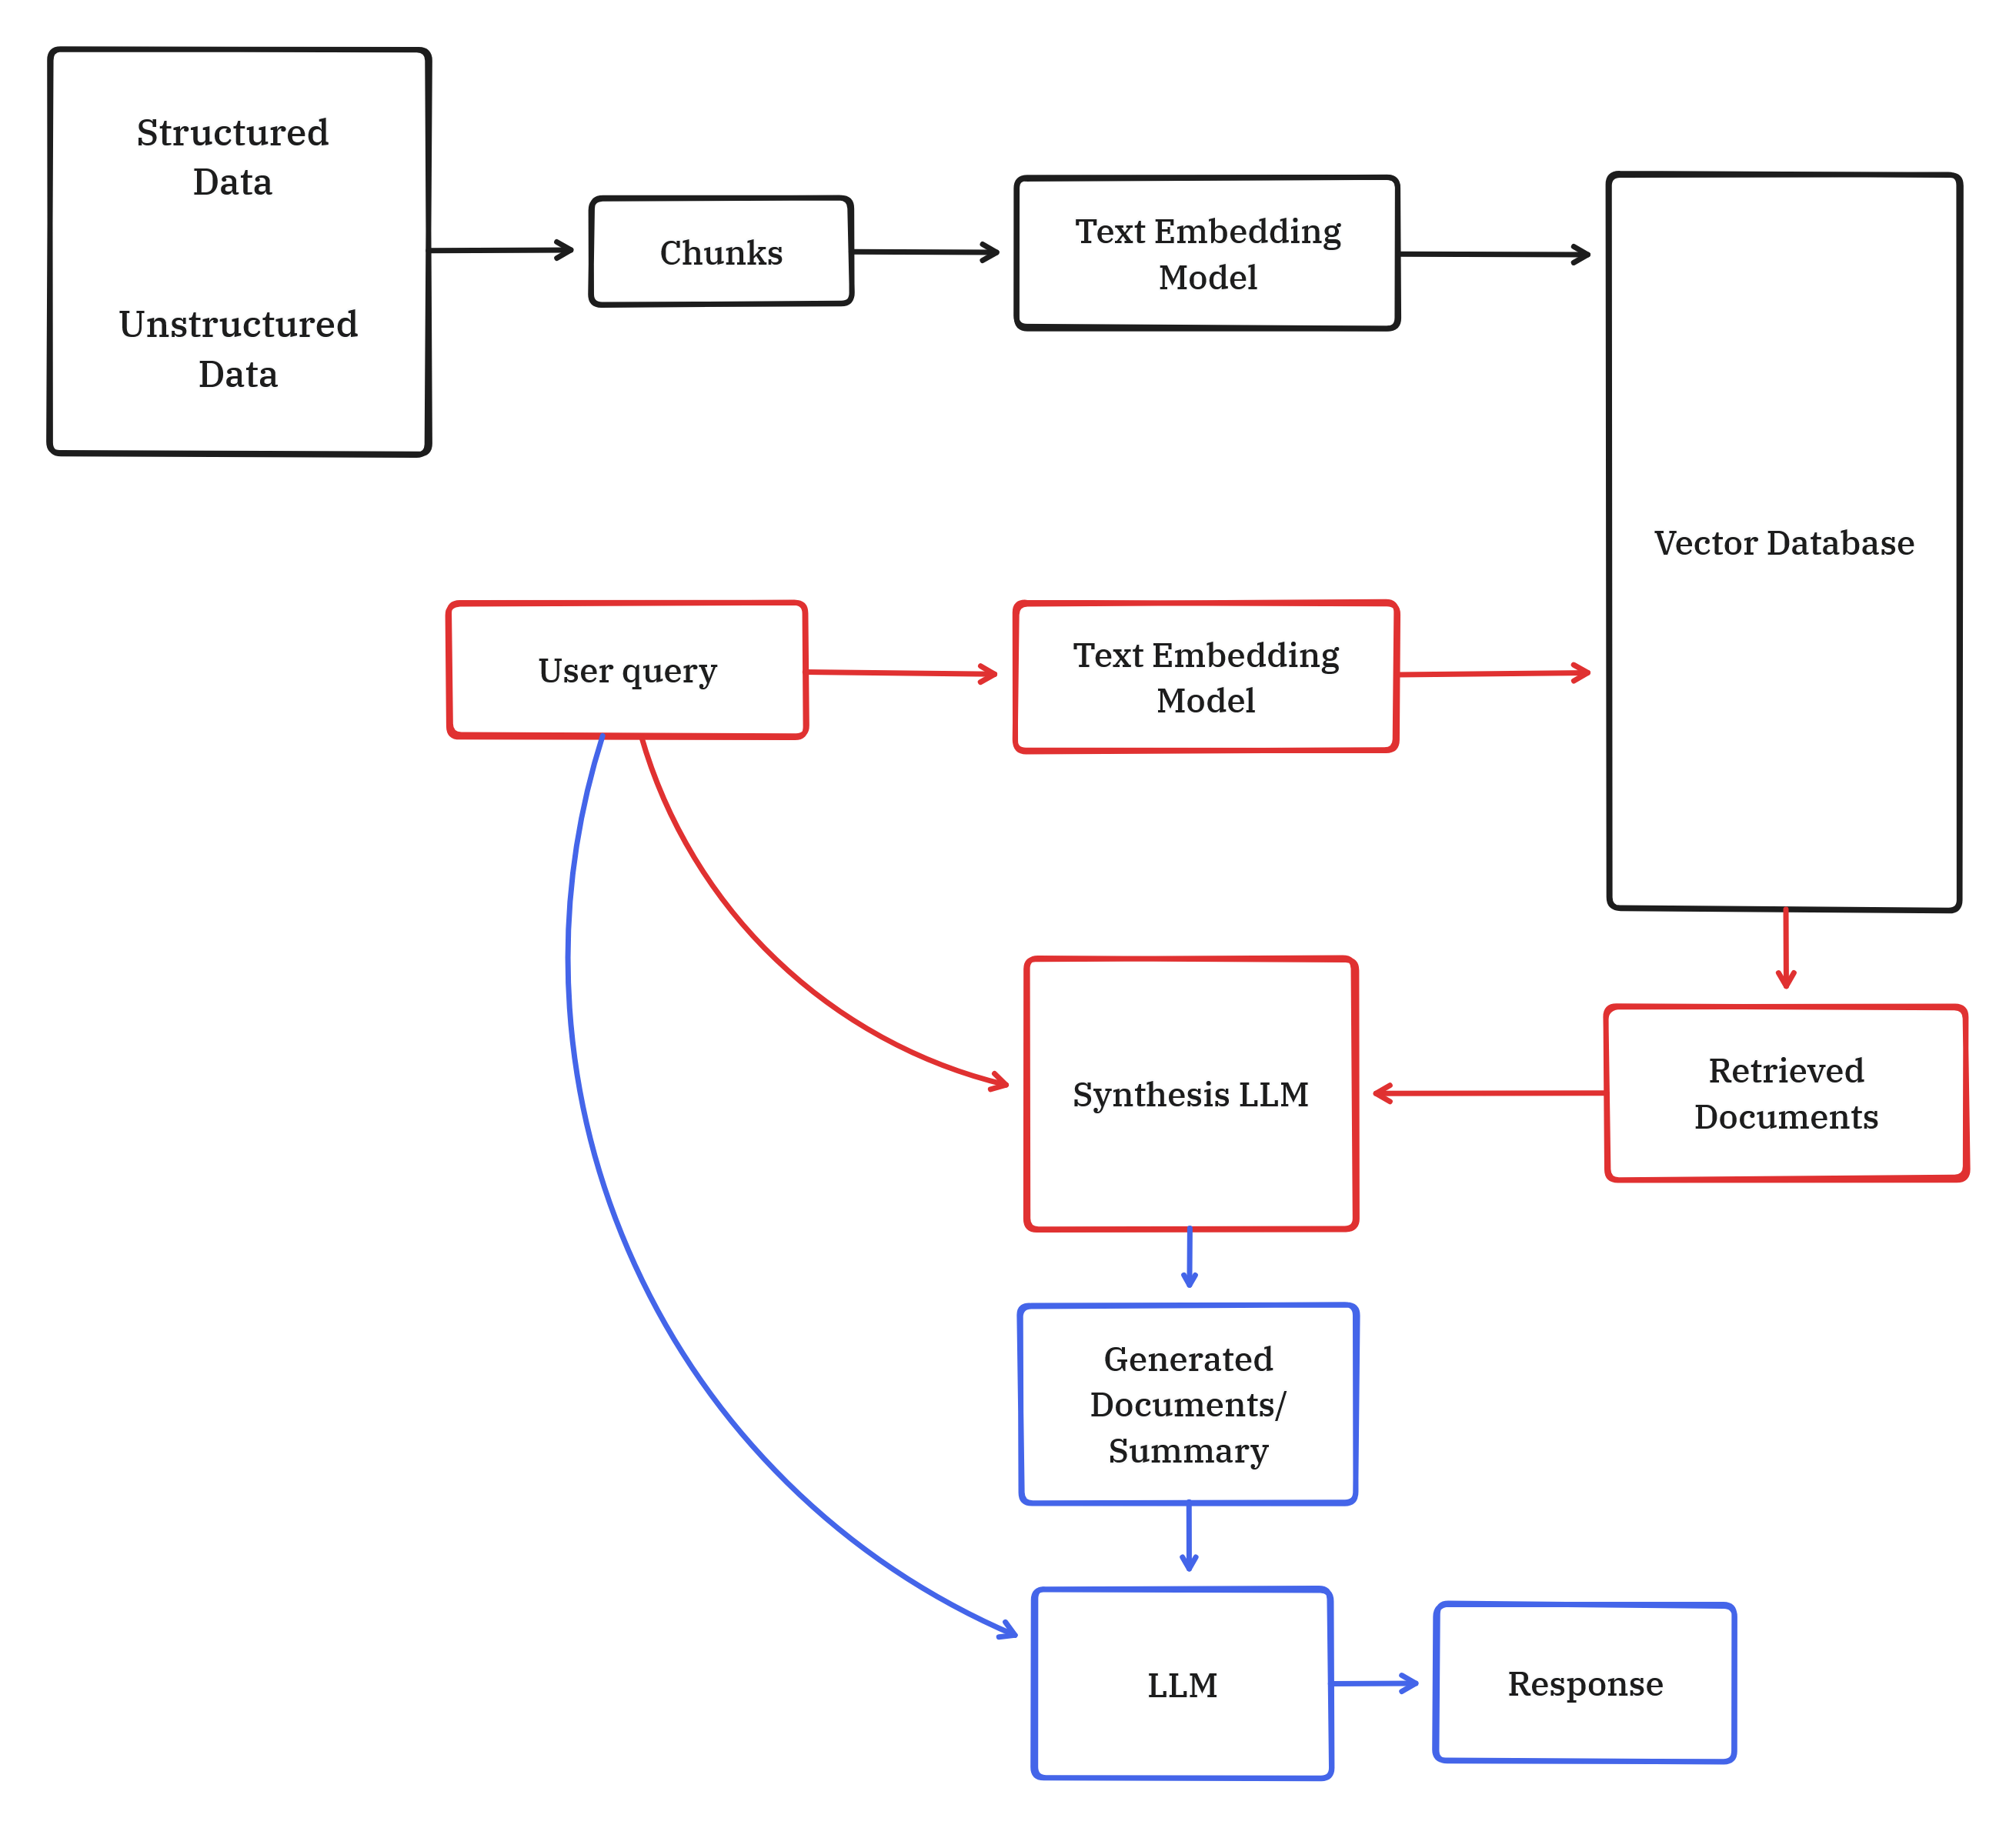
\includegraphics[width=\textwidth]{Synthesis LLM RAG example.png}
	\caption{System Design}
	\centering
	\label{fig:SynthLLMRAG}
\end{figure}

\section{Building the RAG Corpus}
RAG systems can make use of either structured or unstructured data, however in healthcare, data is usually structured.
In order to mimic real healthcare settings, we determined it was necessary to make use of data that was designed for real-world settings.
For our case, we will be making use of a synthetic Fast Healthcare Interoperability Resources (FHIR) dataset, generated and distributed by Synthea \autocite{Synthea2024}.

FHIR is a structured healthcare standard that defines how healthcare information can be shared between different systems regardless of how they are stored.
Individual FHIR patient records are stored in what is known as resources and each resource type represents specific information. A Patient resource would include the patient's name, date of birth, address, etc. Each resource type is specific to its use case.

FHIR records can appear in different file formats, JSON, XML, or RDF. For simpler parsing and handling, we will be making use of JSON FHIR files to build our RAG corpus.

We make use of the open-source library \textit{Llamaindex}\autocite{Liu_LlamaIndex_2022} for abstractions when building the pipeline, as well as creating the database.

\subsection{FHIR Preprocessing}

First, we consider the type of data we wish to embed. JSON files are designed for programmatic use, meaning that they contain many identifying and delimiting tokens. If we were to convert the file in its entirety into its vector representation, it will result in detail being lost due to the repeated embedding of same key-value token pairs. Therefore, we first have to carry out flattening of the FHIR record.

Flattening the FHIR involves two things. First, we must determine what type of information we wish to extract. For this project, we are only working with information from the Patient resource, as well as the Observation, Procedure, Condition, Allergy and MedicationRequest resources. While initially the Encounter resource was used, we decided that it did not add any type of substantial information apart from the reason of the encounter as well as the location where it took place.

\begin{figure}
	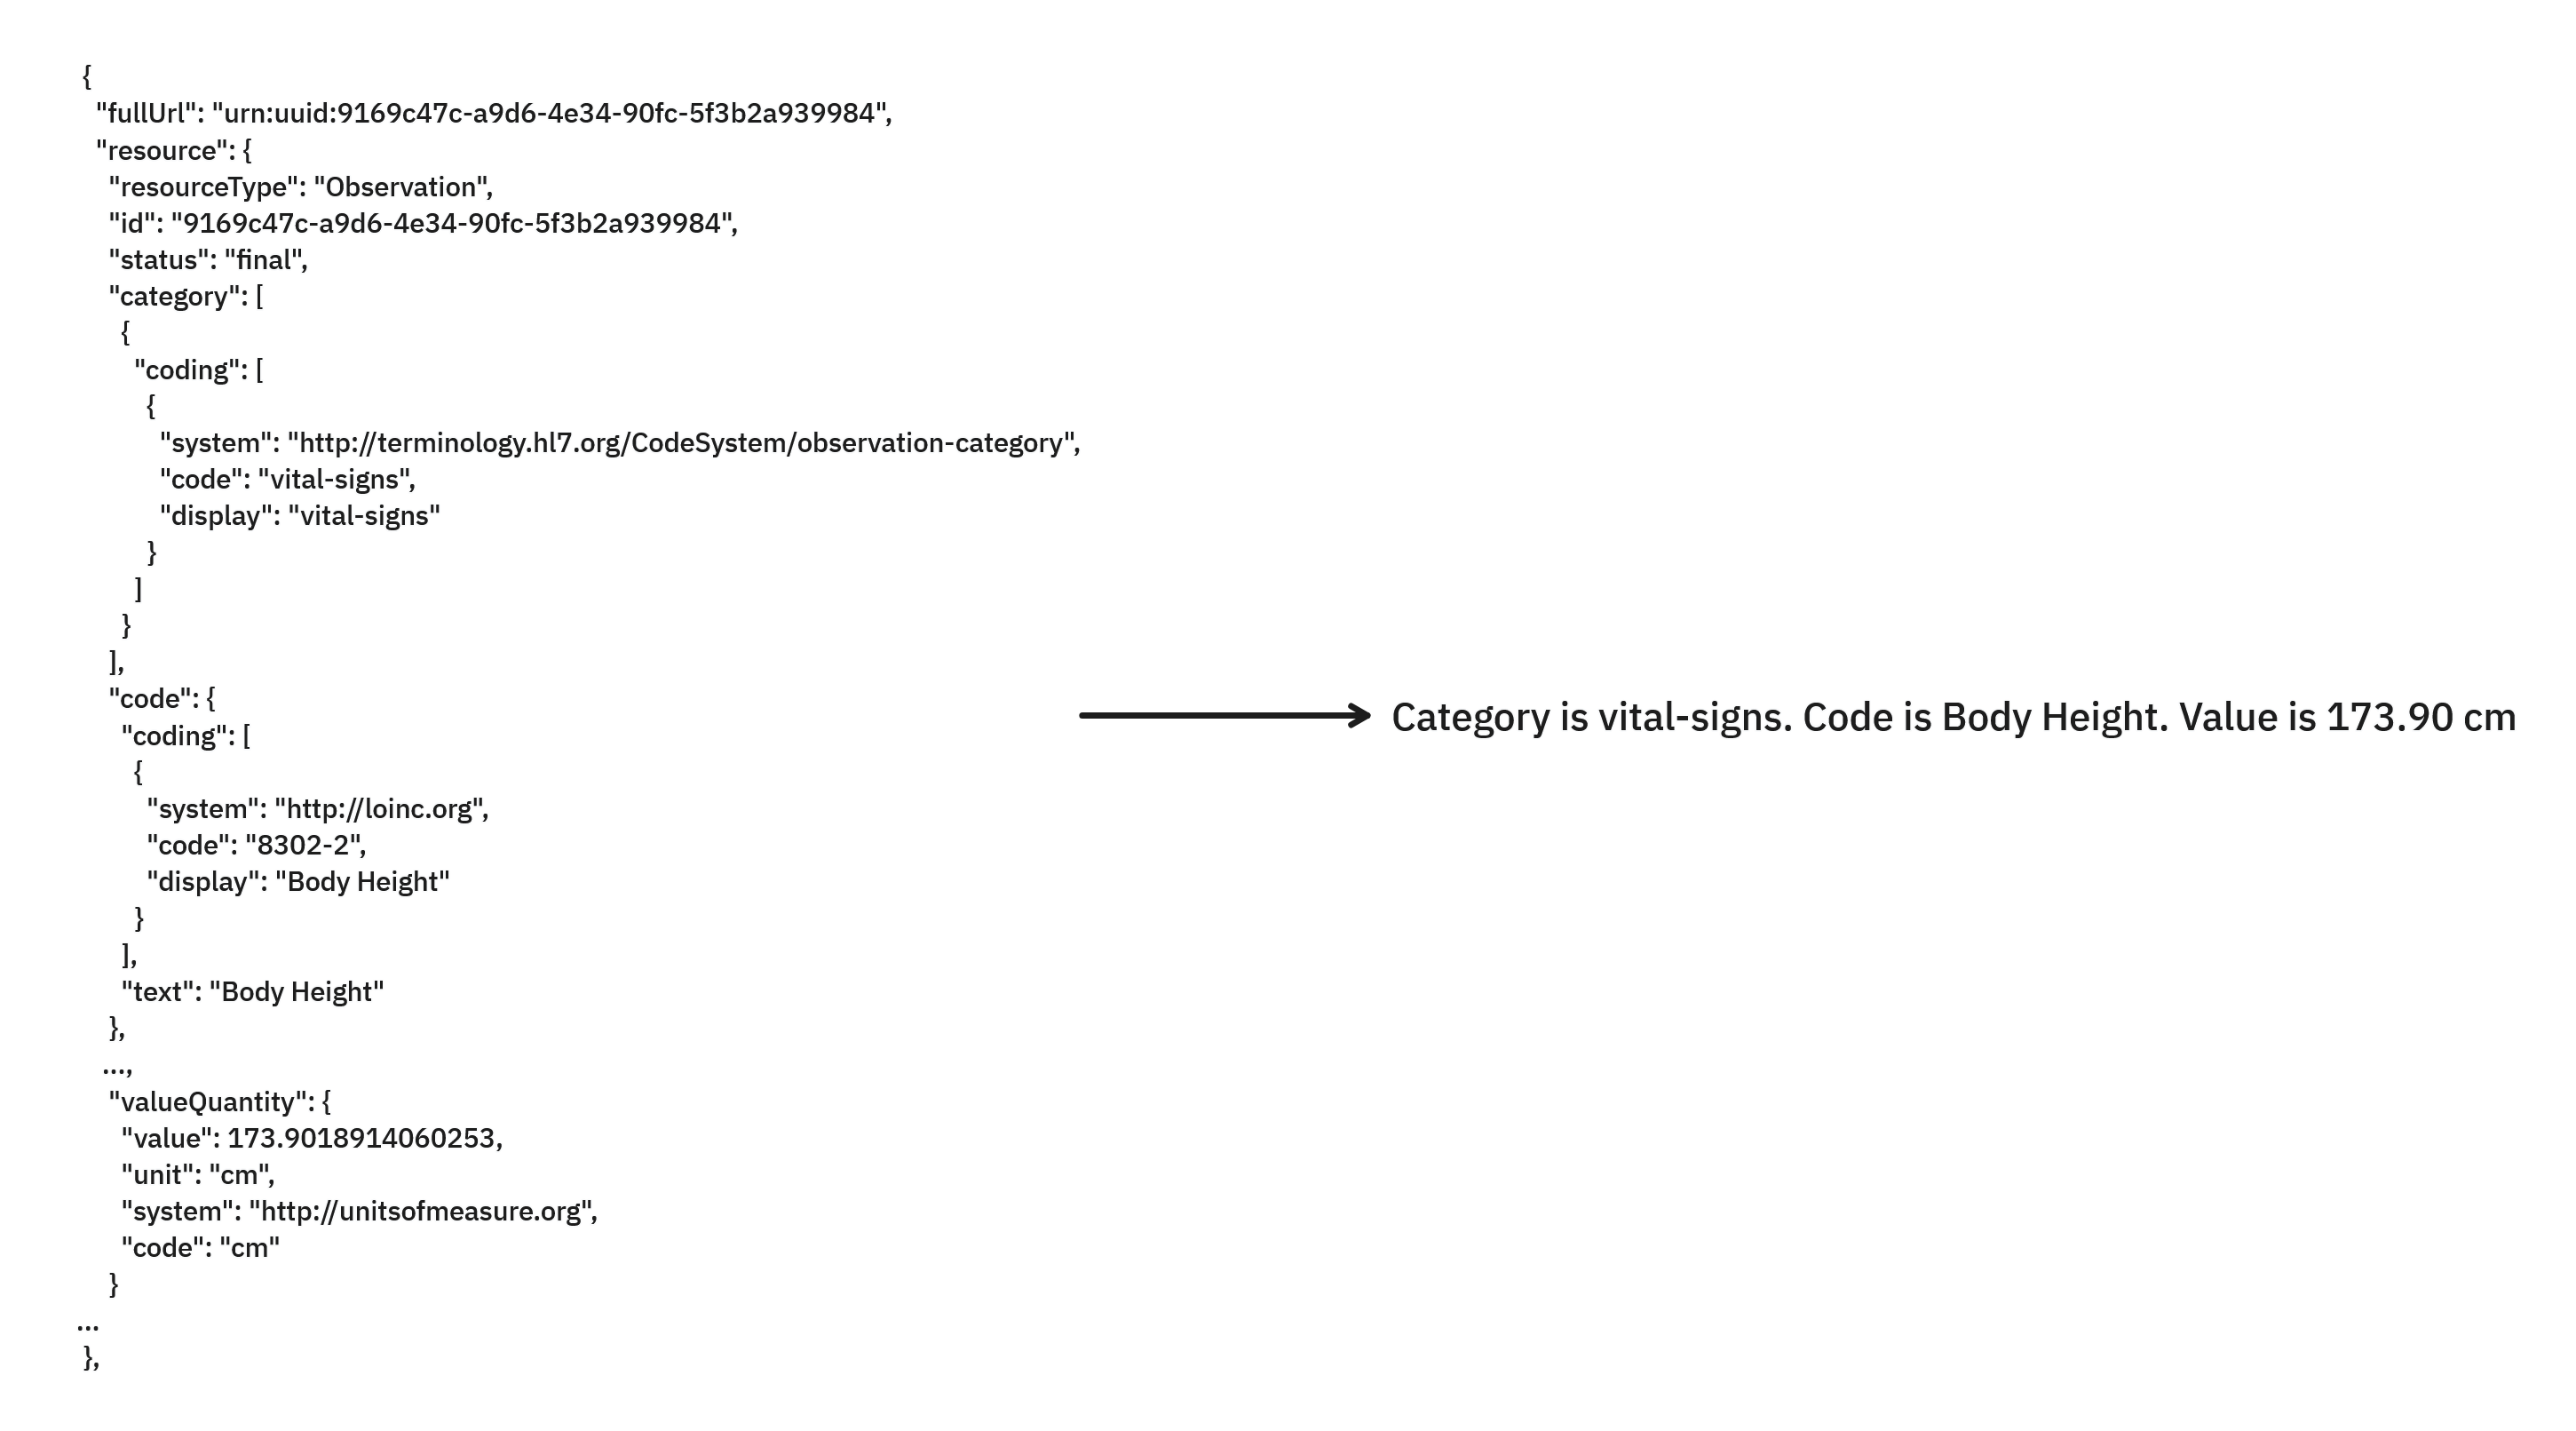
\includegraphics[width=\textwidth]{Converting FHIR to sentence.png}
	\caption{FHIR to sentence}
	\centering
	\label{fig:FHIRtoSentence}
\end{figure}

Secondly, we have to convert the selected information into basic sentences. This is done by recursively un-nesting the FHIR resource with information we specified.
The reason we do this is to improve the embedding accuracy of the FHIR record.
Firstly, we convert FHIR resources to basic sentences.
This is to avoid repeatedly embedding the same key-value token pairs and wasting embedding tokens.
Refer to figure \ref{fig:FHIRtoSentence} for an example.

Processing the FHIR record, we group the information extracted from the Observation and Procedure resources by date. Afterwards, we collate the conditions, allergies, as well as the medications that has been assigned to the patient previously.

Each of these documents are stored in separate files, marked by the patient's name followed by the date of the encounter. These documents are then converted into vectors through the use of a text-embedding model, and stored within a Postgres database utilizing the \textit{pgvector} extension. The embedding model used for generating the embeddings is \emph{bge-base-en-v1.5}. The process is outlined in figure \ref{fig:EmbeddingsDatabase}.


\begin{figure}
	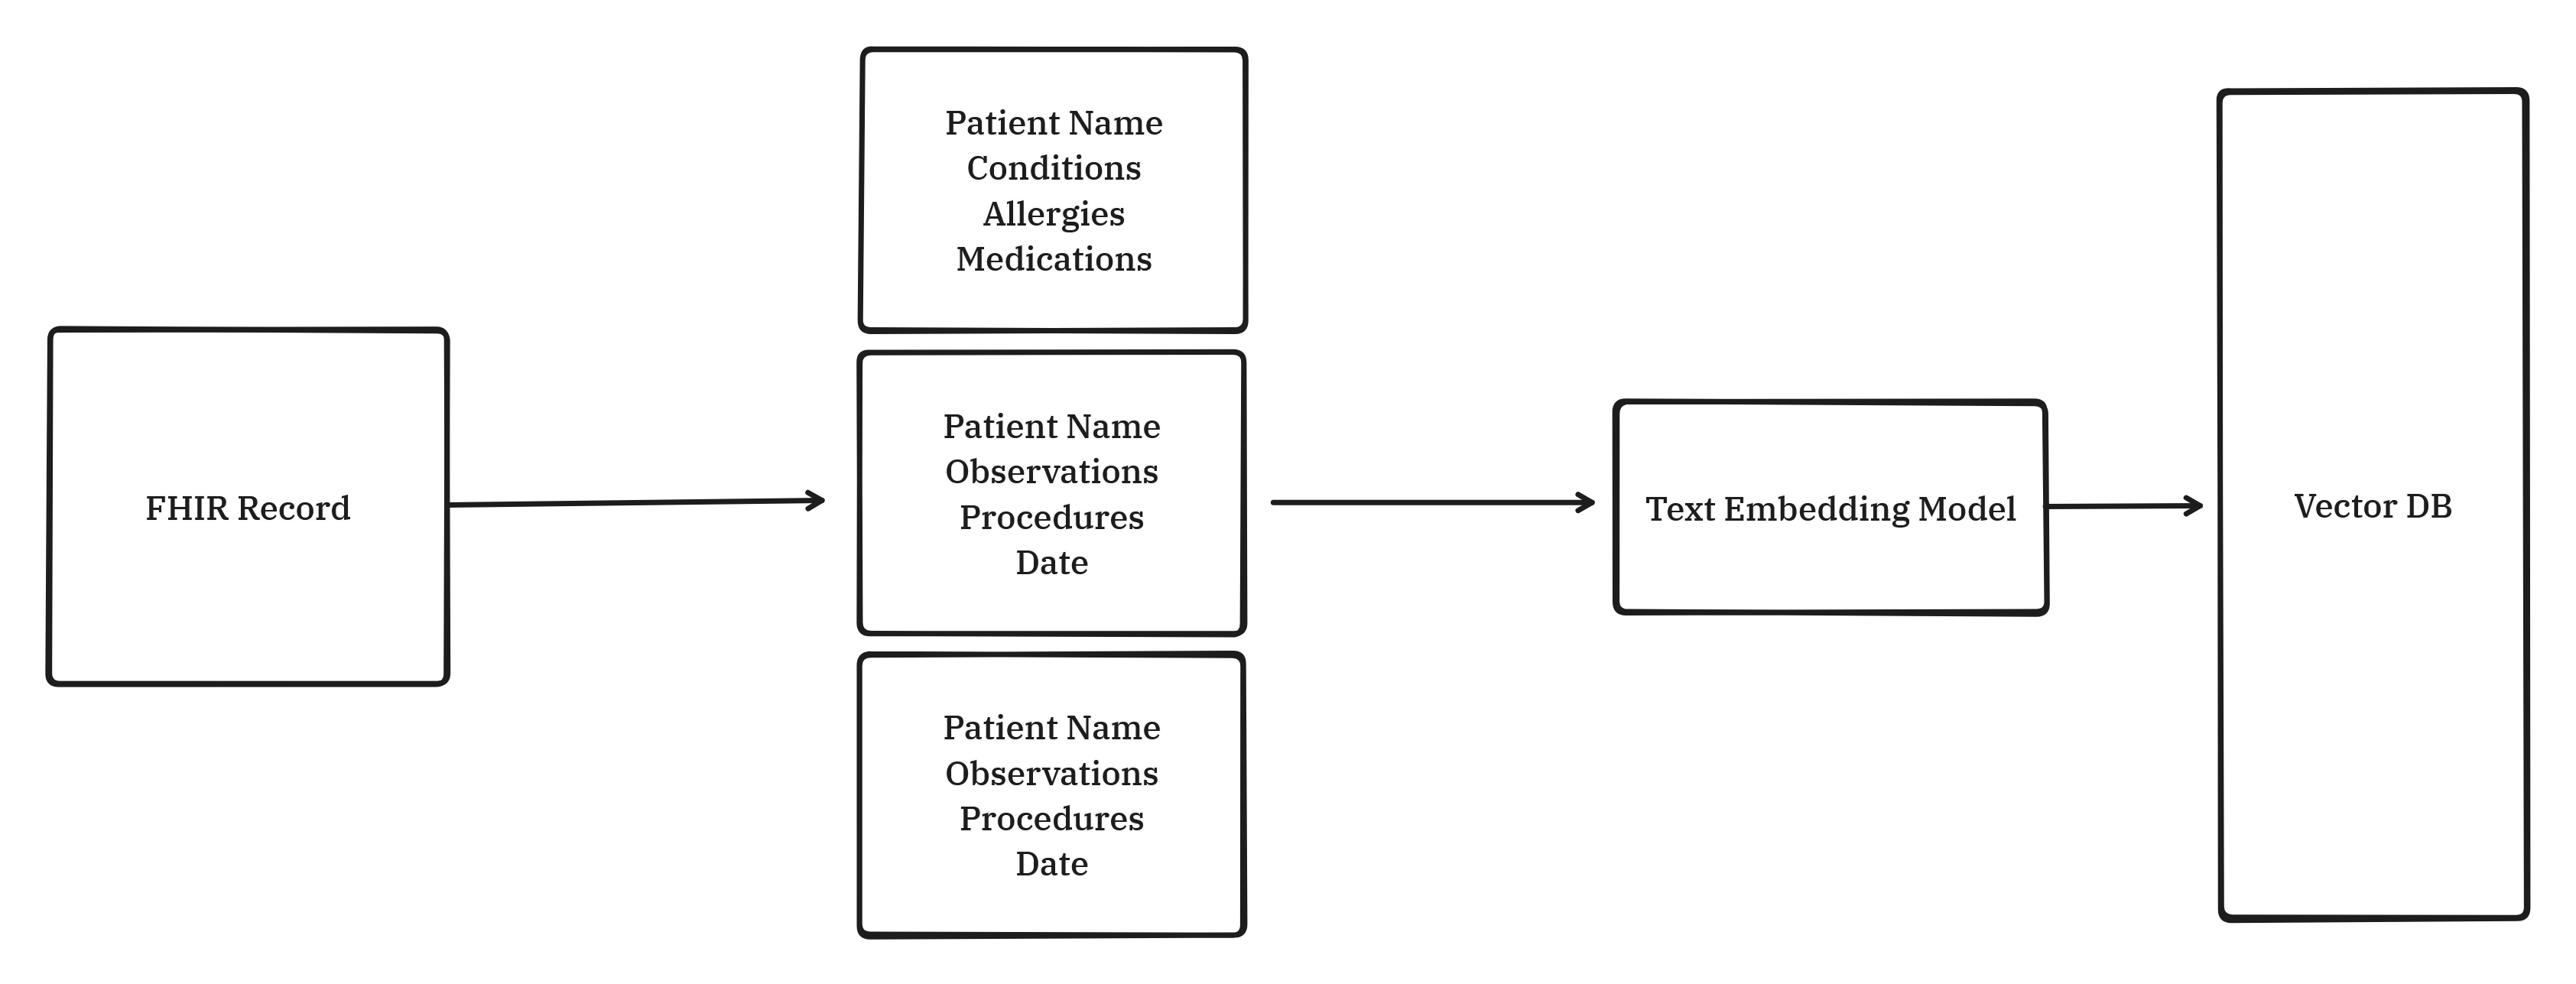
\includegraphics[width=\textwidth]{Store embeddings in DB.png}
	\caption{Embeddings to Database}
	\centering
	\label{fig:EmbeddingsDatabase}
\end{figure}

\subsection{Retrieval}
While not the scope of the project, it should be noted that during the creation of the database, Hierarchical Navigable Small World (HNSW) is used, which plays some influence in the retrieval results. We will not explore how the variations affect the retrieval results in this project.

With the RAG corpus built, we can now move onto retrieving documents associated with a query.
The query goes through the embedding process and its resulting vector is compared to other document vectors in the database.
The top \textit{k} results are returned, with \textit{k} being an adjustable variable.
What determines the chunk's relevance is its cosine similarity to the input query.
Cosine similarity is defined as the following:
\[
	\text{Cosine Similarity} = \cos(\theta) = \frac{\mathbf{A} \cdot \mathbf{B}}{\|\mathbf{A}\| \|\mathbf{B}\|}
\]
and returns a score between 0.0 to 1.0.
Here we can set a minimum cut-off for cosine similarity to adjust the relevance of returned information.
Refer to figure \ref{fig:RetrievalExample} for an example of the returned chunks.

\begin{figure}
	\centering
	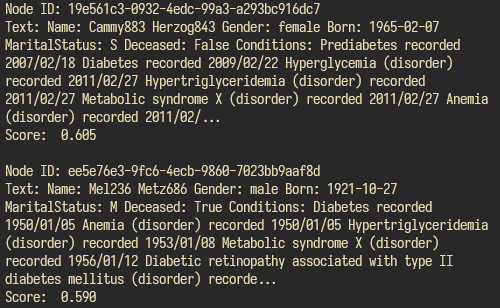
\includegraphics[width=0.5\textwidth]{retrieval example.png}
	\caption{Input Query: Which patients have diabetes?}
	\label{fig:RetrievalExample}
\end{figure}

\section{Large Language Model Choice}

In healthcare settings it is unlikely for a commercial LLM like ChatGPT to see use due to privacy concerns, therefore we make use of a local LLM instead.

Given that we are making use of an agent-based approach, the LLM has to have the capabilities to make use of tools. Tools are, simply put, funcitons that the LLM can call to perform an action. An example would be calling a function for addition or subtraction.

Here we make use of a local LLM instead of a third-party commercial LLM to maintain the idea of privacy. In healthcare settings
\subsection{Synthetic Report Generation}
LLMs differ in capabilities in accordance to their size.
To determine if the chosen LLM (Mistral Nemo 12B) was sufficient for what I needed it to do, I tested its summarization and generation abilities.
Firstly, I merged the previously processed FHIR record for a single patient into a combined document.
This document was then passed to LLM along with a set of instructions.
The specific prompt provided to the LLM is in the appendix, but to summarize:
\begin{itemize}
	\item Break the summary into clear sections with headers
	\item Include exact numerical values
	\item Use precise dates
	\item Report conditions with specific terminology
	\item Summarize readings into a range spanning from min-max
\end{itemize}

The generated report summary was then passed to the LLM with instructions to anonymize information by rounding values as well as removing ages, dates, and names.
This was done for three different types of prompting strategies, Zero-Shot, Chain-of-Thought, and Structured Output.

Refer to figure \ref{fig:SynthSummary} for a side-by-side comparison for Zero-Shot generation.
Full results for each are present in the appendix.
Overall, the LLM was effective in following instructions as well as working with a large amount of context.

\begin{figure}
	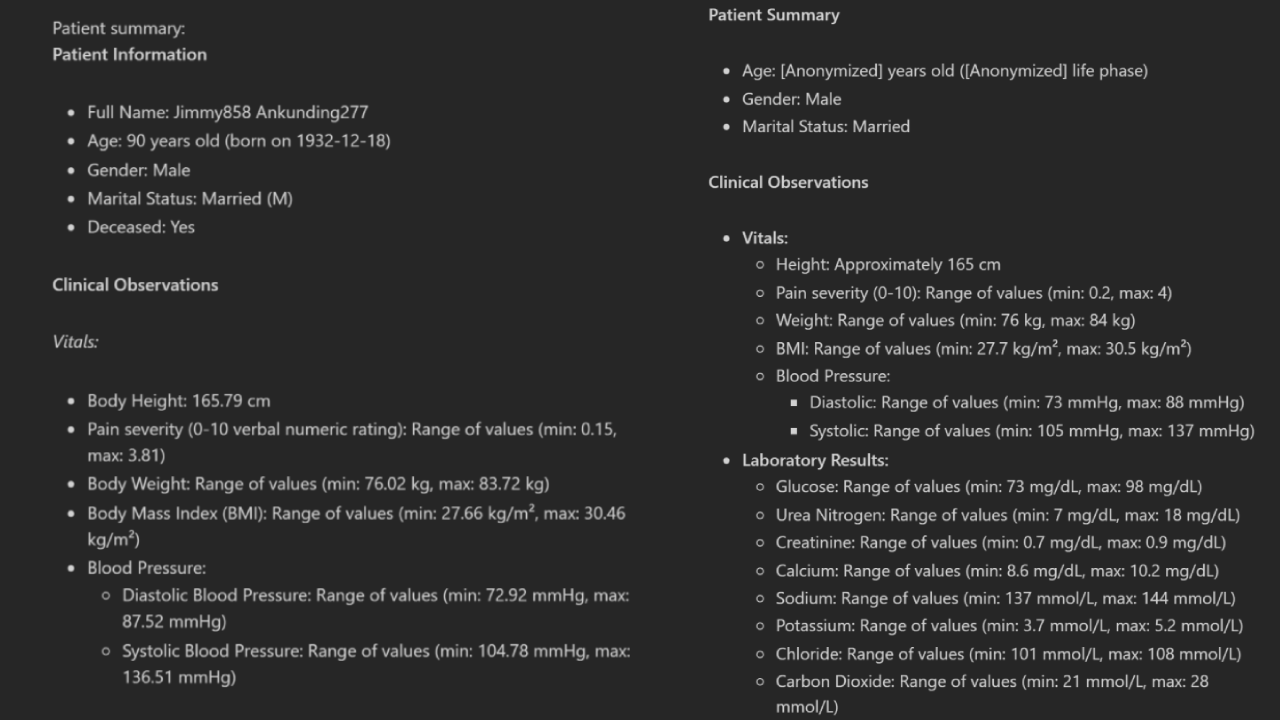
\includegraphics[width=\textwidth]{Zero-shot-summary-vs-synth.png}
	\centering
	\caption{Zero-Shot Generated Summary V.S. Synthesized Summary}
	\label{fig:SynthSummary}
\end{figure}
